\subsection{SN-DCGAN}
\label{sec:exp-sndcgan}
We implement the spectral normalization layer and use on the discriminator of the DCGAN used in the previous section. We present the evolution of the inception score and losses in Figures \ref{fig:exp-sndcgan-is} and \ref{fig:exp-sndcgan-losses}, respectively.
   
% is
\begin{figure}[h]
\centering
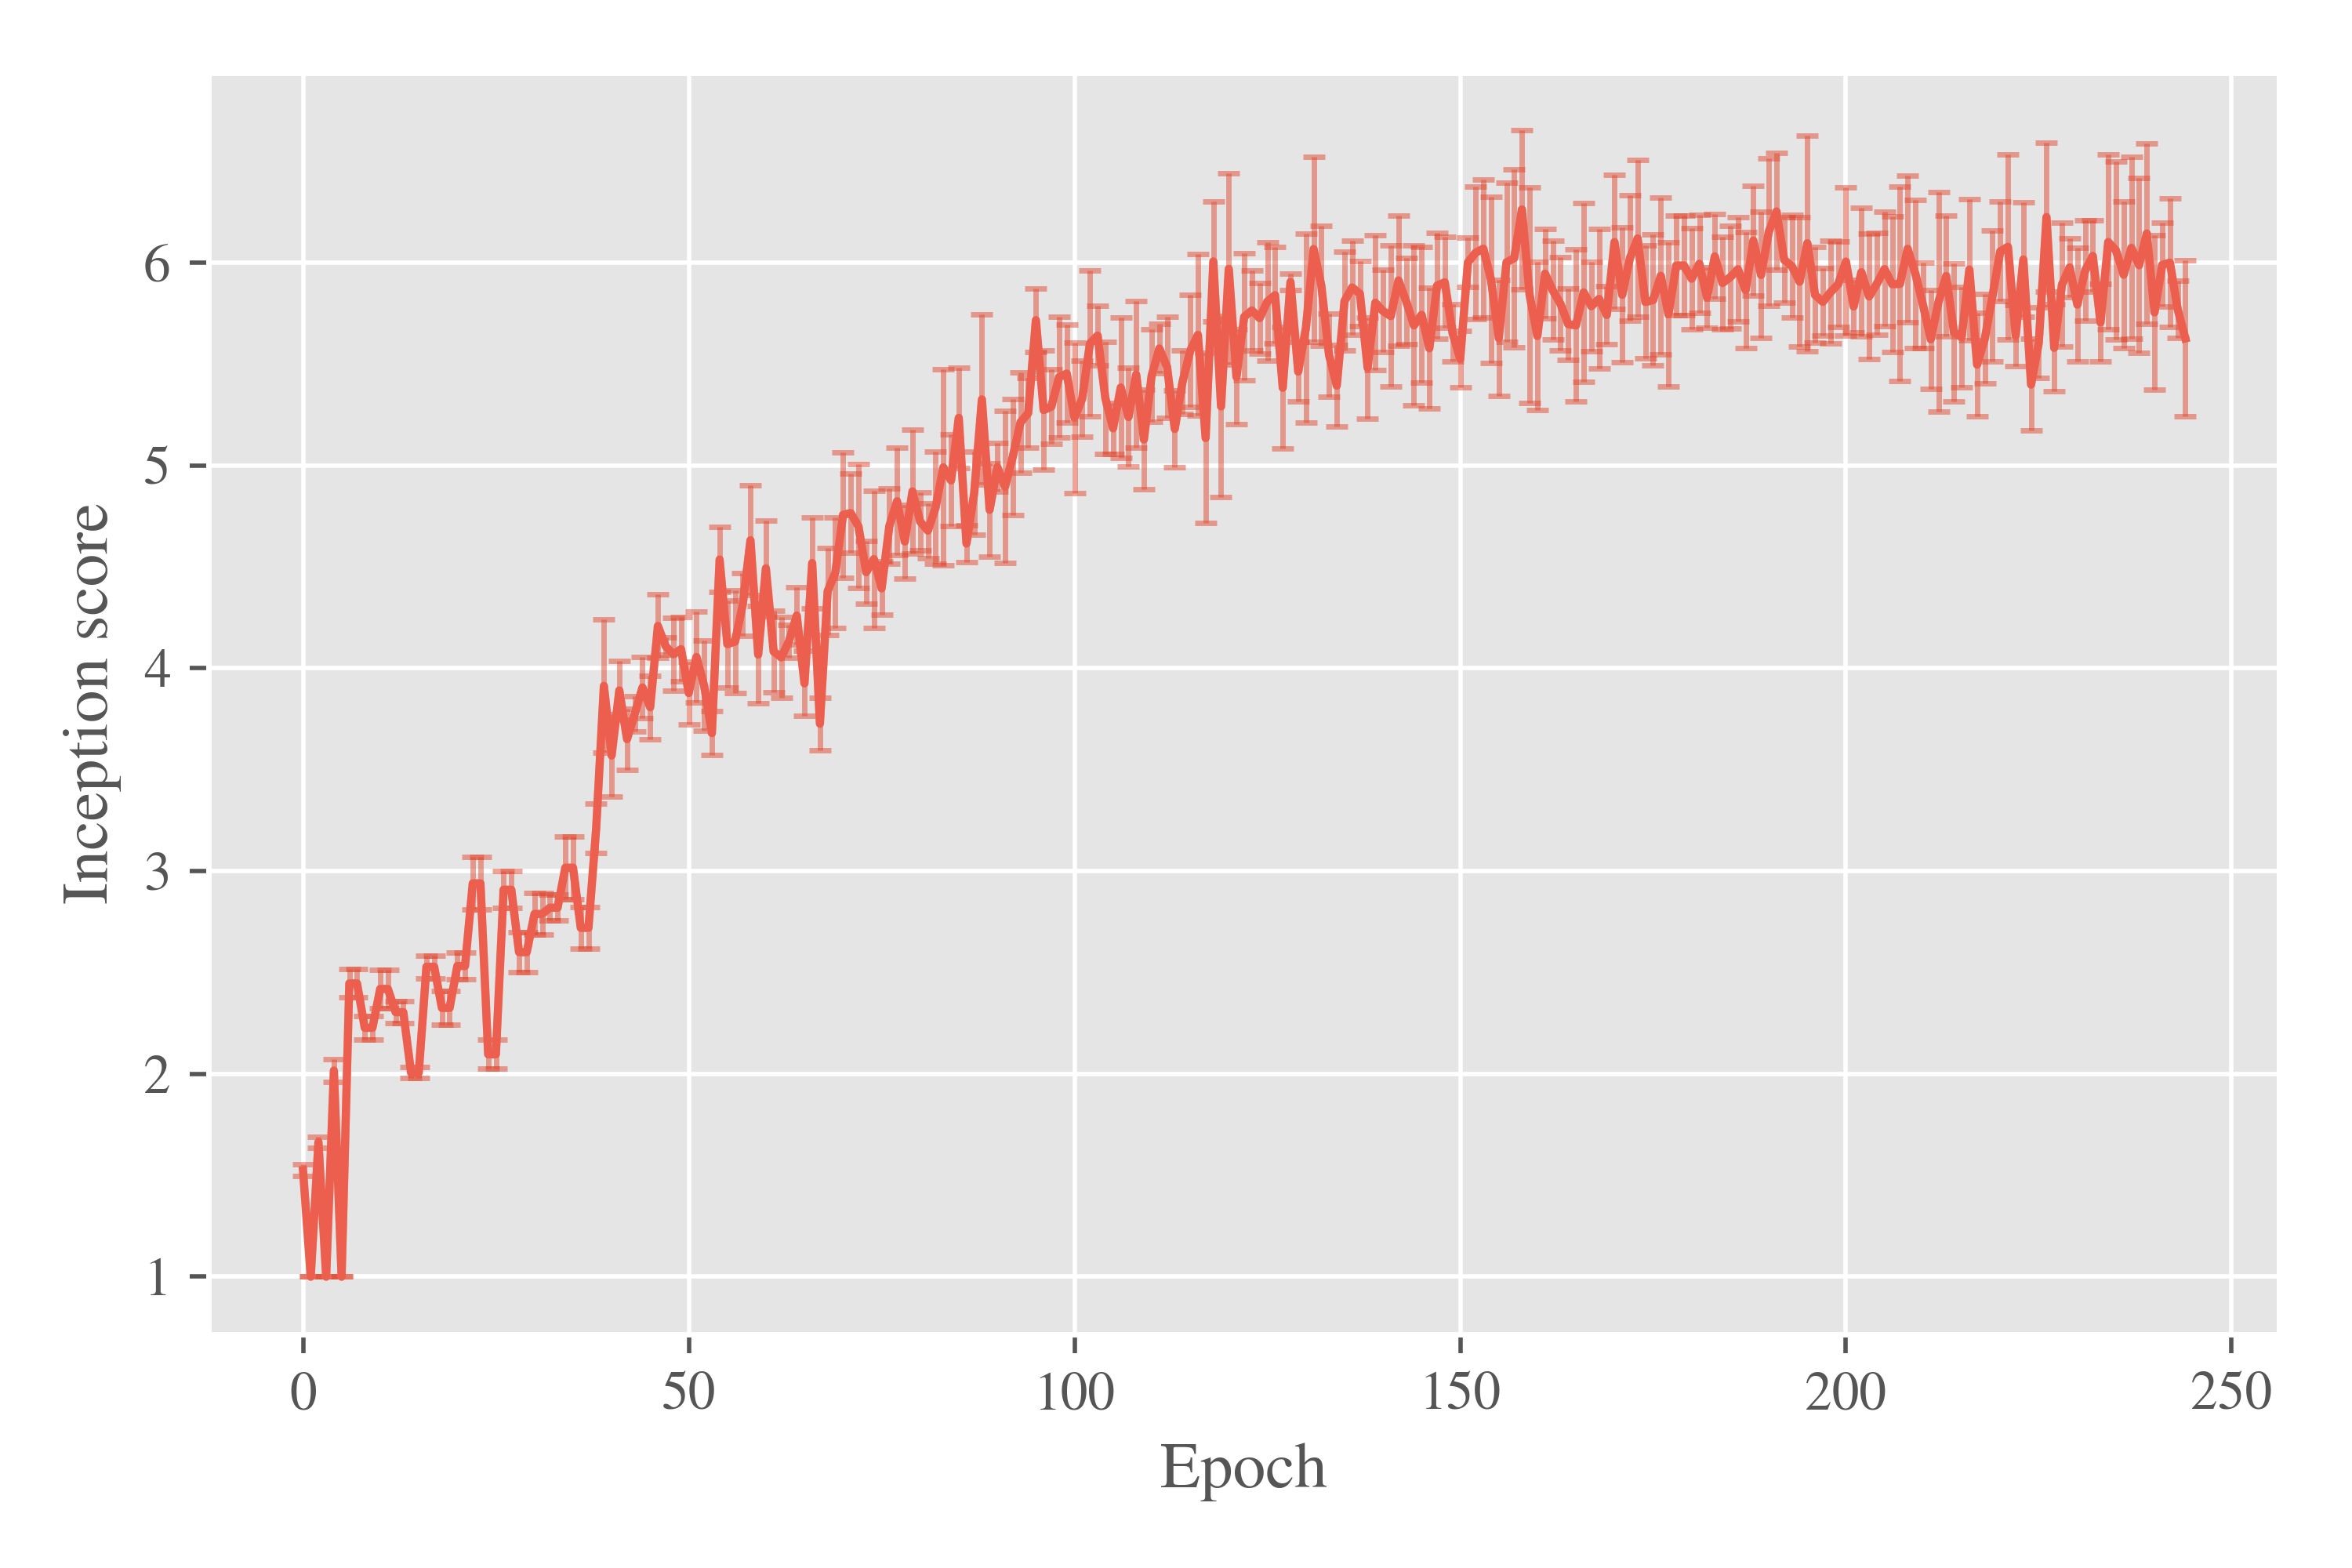
\includegraphics[width=\textwidth]{../code/results/figures/sndcgan_cifar10_is.png}
\caption{SN-DCGAN - Inception score, training on cifar10 over ~250 epochs}
\label{fig:exp-sndcgan-is}
\end{figure}
We don't notice any significant improvement on the mean of the inception score after convergence. However, the average standard deviation is reduced compared to that of the DCGAN without spectral normalization, depicted in Figure \ref{fig:exp-dcgan-is}.
% losses
\begin{figure}[h]
\centering
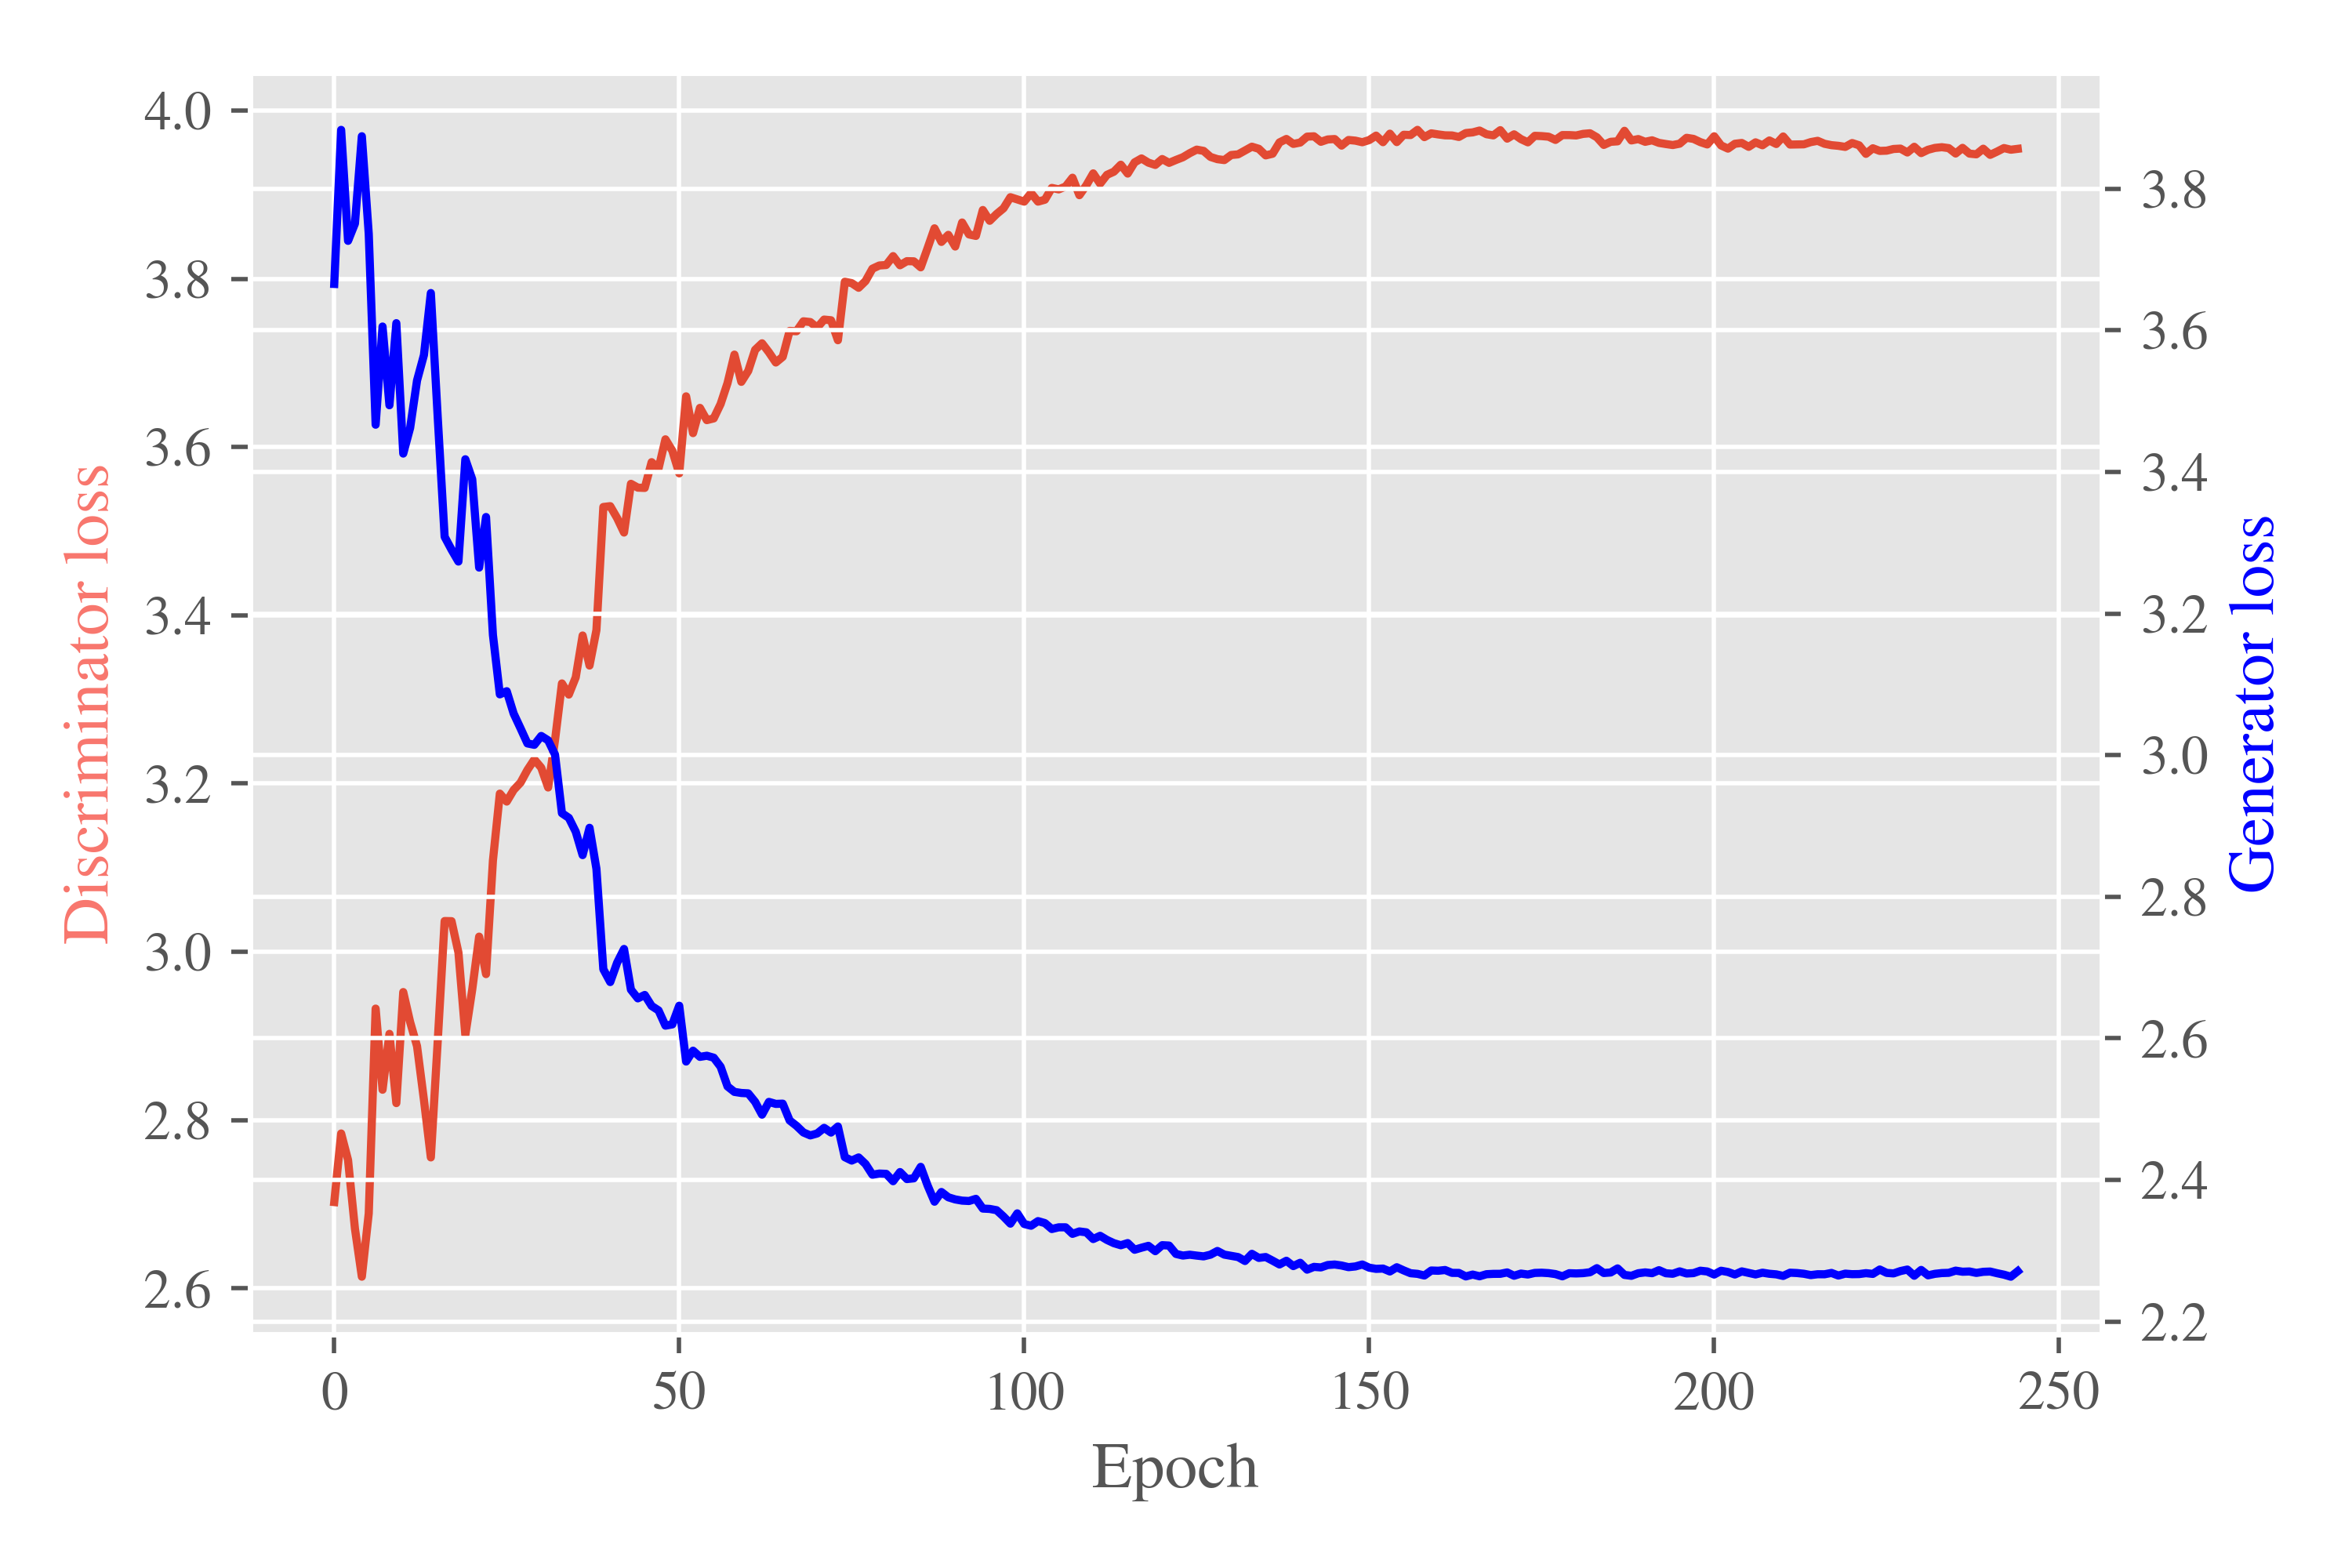
\includegraphics[width=\textwidth]{../code/results/figures/sndcgan_cifar10_losses.png}
\caption{SN-DCGAN - Losses training on cifar10 over ~250 epochs.}
\label{fig:exp-sndcgan-losses}
\end{figure}
In Figure \ref{fig:exp-dcgan-losses}, we observe that both losses are much smoother with spectral normalization. This is the desired result; the original intent of the paper on spectral normalization was to provide a solution to stabilize the training of GANs \cite{miyato2018spectral}. 